\documentclass[aspectratio=169]{beamer}

% ======================================================================
% Theme & appearance
% ======================================================================
\usetheme{Madrid}
\usecolortheme{whale}

\usepackage[utf8]{inputenc}
\usepackage{graphicx}
\usepackage{booktabs}
\usepackage{amsmath}
\usepackage{amssymb}
\usepackage{tikz}
\usepackage{array}
\usepackage{tabularx}
\usepackage{hyperref}
\usepackage{xcolor}

% Image path
\graphicspath{{images/}}

% Frame title / section styling
\setbeamertemplate{navigation symbols}{}
\setbeamercolor{title}{fg=black}

% Title page
\title{NORMALIZED CUTS \\ \& IMAGE SEGMENTATION}
\author{Jianbo Shi and Jitendra Malik (2000)}
\date{}

\begin{document}

% ======================================================================
% SLIDE 1 -- Title
% ======================================================================
\begin{frame}
    \titlepage
    \vspace{0.5cm}
    \centering
    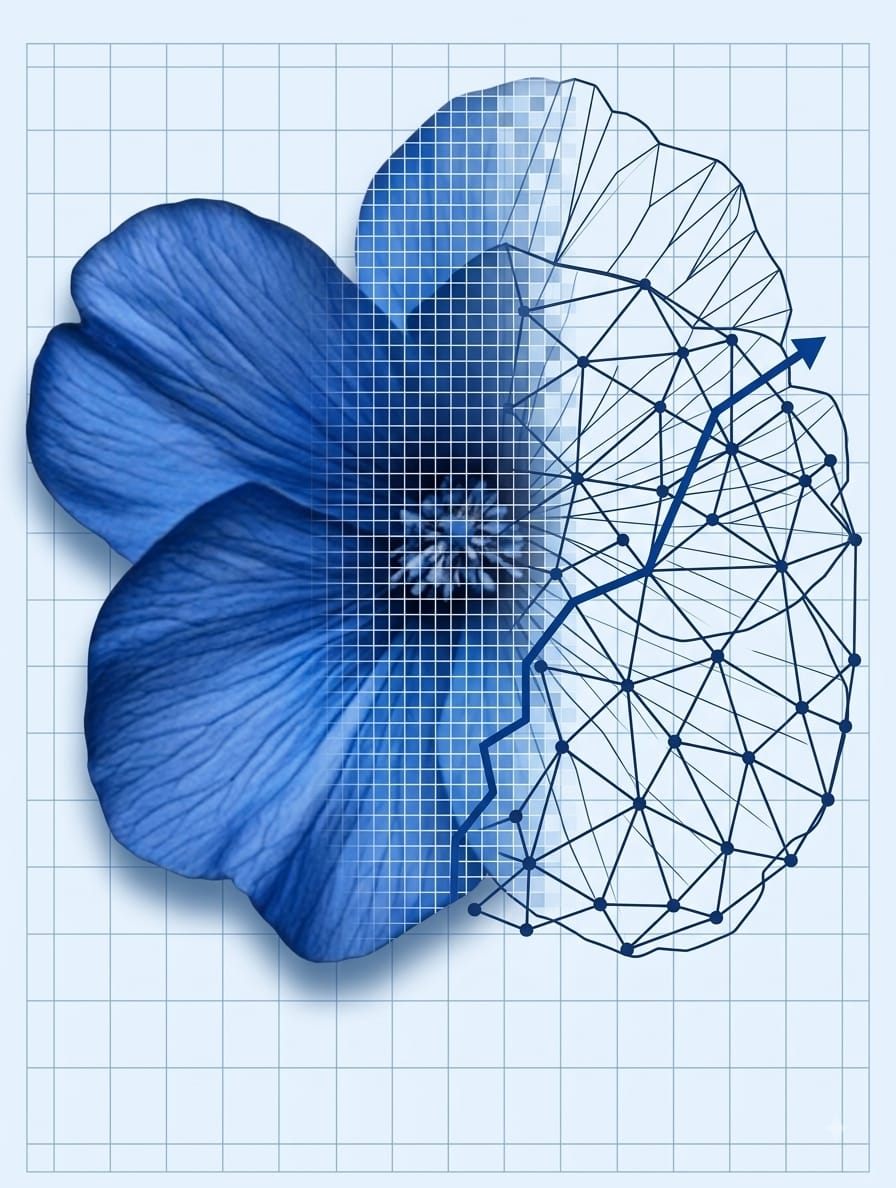
\includegraphics[width=0.35\textwidth]{slide1_title_bg.jpg}
\end{frame}

% ======================================================================
% SLIDE 2 -- Abstract
% ======================================================================
\begin{frame}{Abstract}

    \small
    \textbf{A New Perspective on Segmentation}

    \begin{itemize}
        \item The paper proposes a novel global approach to solve the perceptual grouping problem in vision by capturing an image's overall structure rather than focusing on local features.
        \item Instead of focusing on local pixel features, Shi and Malik emphasize on extracting the global impression of the image.
        \item Image segmentation is treated as a graph partitioning problem using a new global criterion called the \textbf{normalized cut}.
        \item This measures \textbf{both, the} total dissimilarity between the different groups as well as the total similarity within the groups.
        \item Along with this, they have also shown an efficient computational technique based on generalized eigenvalue problem that can be used to optimize this criterion.
    \end{itemize}

\end{frame}

% ======================================================================
% SLIDE 3 -- Grouping as graph partitioning
% ======================================================================
\begin{frame}{Grouping as graph partitioning}

    \small
    \textbf{Graph Representation}

    \begin{itemize}
        \item An image is treated as a weighted undirected graph $G = (V, E)$.
        \begin{itemize}
            \item \textbf{Nodes ($V$):} Pixels of the image.
            \item \textbf{Edges ($E$):} Connections between every pair of nodes.
            \item \textbf{Weight ($w_{ij}$):} Similarity between nodes $i$ and $j$ based on spatial proximity and feature (intensity, color, brightness etc).
        \end{itemize}
    \end{itemize}

    \begin{columns}
        \begin{column}{0.35\textwidth}
            
\includegraphics[width=0.45\textwidth]{slide3_graph_nodes.png}
            
\includegraphics[width=0.45\textwidth]{slide3_graph_edges.png}\\[0.2em]
            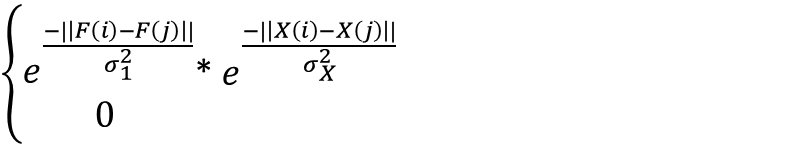
\includegraphics[width=0.45\textwidth]{slide3_graph_weight.png}
            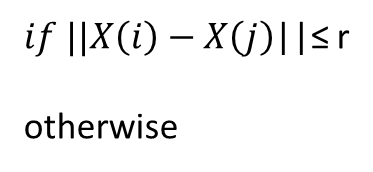
\includegraphics[width=0.45\textwidth]{slide3_partition_goal.png}
        \end{column}
        \begin{column}{0.65\textwidth}
            \textbf{THE PARTITIONING GOAL}\par\vspace{0.1em}
            {\footnotesize The core objective is to partition the graph into disjoint sets such that the similarity within sets (intra-cluster) is high, and the similarity across different sets (inter-cluster) is low.}

            {\footnotesize
            $w(i,j) =
            \begin{cases}
                e^{-\frac{\lVert F(i)-F(j)\rVert^2}{\sigma_I^2}}
                \cdot e^{-\frac{\lVert X(i)-X(j)\rVert^2}{\sigma_X^2}}
                & \text{if } \lVert X(i)-X(j)\rVert < r,\\
                0 & \text{otherwise}.
            \end{cases}$
            \\[0.2em]
            where $X(i)$: spatial location of $i$, $F(i)$: feature of $i$.
            }
        \end{column}
    \end{columns}

\end{frame}

% ======================================================================
% SLIDE 4 -- THE MIN-CUT
% ======================================================================
\begin{frame}{The Min-Cut}

    \begin{itemize}
        \item Traditional minimum cut algorithms aim to minimize \textbf{cut cost}.
        \item However, this heavily biases the algorithm toward cutting small sets of isolated nodes, failing to capture the global structure of the image.
    \end{itemize}

    \[
        \mathrm{Cut}(A, B) = \sum_{u \in A,\, v \in B} w(u, v)
    \]

    \begin{columns}
        \begin{column}{0.4\textwidth}
            \textbf{Optimal cut} \quad \textbf{Min cut result}
            \begin{figure}
                \centering
                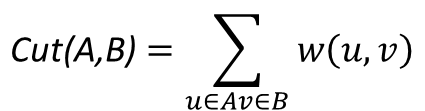
\includegraphics[width=0.55\textwidth]{slide4_min_cut.png}
            \end{figure}
        \end{column}
        \begin{column}{0.6\textwidth}
            \begin{itemize}
                \item Min-Cut favors cutting small sets of isolated nodes, as the absolute sum of edge weights is naturally smaller for fewer nodes.
                \item This fails to capture the global structure of the image which makes the final segmentation absolutely meaningless.
            \end{itemize}
        \end{column}
    \end{columns}

\end{frame}

% ======================================================================
% SLIDE 5 -- THE MATHEMATICAL SOLUTION (NCut)
% ======================================================================
\begin{frame}{The Mathematical Solution}

    \textbf{NCut: Normalized Cut Value --- Balancing the Cut}

    \begin{itemize}
        \item To avoid unnatural bias for partitioning out small regions, Shi and Malik proposed the Normalized Cut (NCut). It computes the cut cost as a fraction of the total edge connections to all nodes in the graph.
    \end{itemize}

    \begin{columns}
        \begin{column}{0.5\textwidth}
            \begin{figure}
                \centering
                
\includegraphics[width=0.8\textwidth,height=0.28\textheight,keepaspectratio]{slide5_ncut_formula.png}
            \end{figure}
        \end{column}
        \begin{column}{0.5\textwidth}
            \begin{itemize}
                \item $\mathrm{assoc}(A, V)$: the total connection from nodes in $A$ to all nodes in the entire graph.
                \item $\mathrm{assoc}(B, V)$: the total connection from nodes in $B$ to all nodes in the entire graph.
                \item Minimizing \textbf{Ncut} is equivalent to increasing the \textbf{association}, thus making sure that we don't isolate a single pixel.
            \end{itemize}
        \end{column}
    \end{columns}

    \begin{figure}
        \centering
        
\includegraphics[width=0.5\textwidth,height=0.25\textheight,keepaspectratio]{slide5_ncut_example.png}
    \end{figure}

\end{frame}

% ======================================================================
% SLIDE 6 -- THE MATHEMATICAL SOLUTION (Nassoc)
% ======================================================================
\begin{frame}{The Mathematical Solution}

    Minimizing the dissimilarity between partitions is mathematically equivalent to maximizing the within-cluster similarity.

    \textbf{Normalized Association}
    \[
        \mathrm{Nassoc}(A, B) = \frac{\mathrm{assoc}(A, A)}{\mathrm{assoc}(A, V)} + \frac{\mathrm{assoc}(B, B)}{\mathrm{assoc}(B, V)}
    \]

    \textbf{Relation between normalized cut and normalized association}
    \[
        \mathrm{Ncut}(A, B) + \mathrm{Nassoc}(A, B) = 1
    \]

    \begin{itemize}
        \item \textbf{Ncut($A$,$B$) decreases as Nassoc($A$,$B$) increases}.
        \item $\mathrm{assoc}(A, A)$ and $\mathrm{assoc}(B, B)$ are total weights of edges connecting nodes within $A$ and $B$ respectively.
    \end{itemize}

    \begin{columns}
        \begin{column}{0.33\textwidth}
            
\includegraphics[width=\textwidth,height=0.22\textheight,keepaspectratio]{slide6_nassoc_formula1.png}
        \end{column}
        \begin{column}{0.33\textwidth}
            
\includegraphics[width=\textwidth,height=0.22\textheight,keepaspectratio]{slide6_nassoc_formula2.png}
        \end{column}
        \begin{column}{0.33\textwidth}
            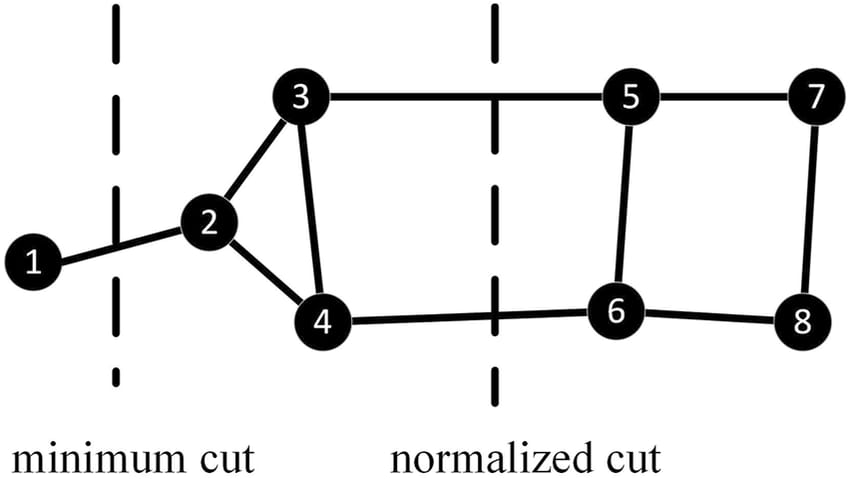
\includegraphics[width=\textwidth,height=0.22\textheight,keepaspectratio]{slide6_ncut_nassoc_relation.jpg}
        \end{column}
    \end{columns}

\end{frame}

% ======================================================================
% SLIDE 7 -- Mathematical formulation
% ======================================================================
\begin{frame}{Mathematical Formulation}

    Minimizing \textbf{Ncut} is an \emph{\textbf{NP hard problem}}. However, it can be transformed into a generalized eigenvalue system.

    \emph{\textbf{W: Affinity matrix (similarities).}}
    \[
        w_{ij} =
        \begin{cases}
            e^{-\frac{\lVert F(i)-F(j)\rVert^2}{\sigma_I^2}}
            \cdot e^{-\frac{\lVert X(i)-X(j)\rVert^2}{\sigma_X^2}}
            & \text{if } \lVert X(i)-X(j)\rVert < r,\\
            0 & \text{otherwise}.
        \end{cases}
    \]

    \emph{\textbf{D: Diagonal matrix.}}
    \[
        D_{ii} = d_i = \sum_j w_{ij}
    \]

    \emph{\textbf{The second smallest eigenvector of this system provides us the optimal partition.}}

    \begin{columns}
        \begin{column}{0.5\textwidth}
            
\includegraphics[width=0.5\textwidth,height=0.16\textheight,keepaspectratio]{slide7_eigen_system.png}
            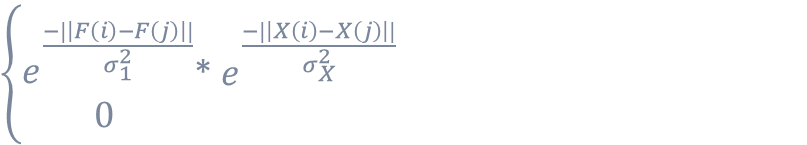
\includegraphics[width=0.5\textwidth,height=0.16\textheight,keepaspectratio]{slide7_affinity_formula.png}
        \end{column}
        \begin{column}{0.5\textwidth}
            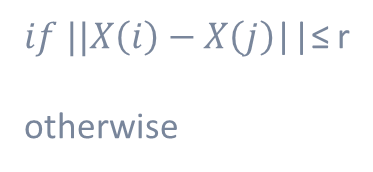
\includegraphics[width=0.5\textwidth,height=0.16\textheight,keepaspectratio]{slide7_diagonal_formula.png}
            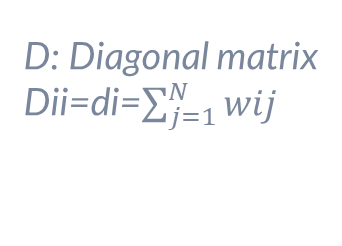
\includegraphics[width=0.5\textwidth,height=0.16\textheight,keepaspectratio]{slide7_eigenvalue.png}
        \end{column}
    \end{columns}

\end{frame}

% ======================================================================
% SLIDE 8 -- Grouping Algorithm: Step 1
% ======================================================================
\begin{frame}{The Grouping Algorithm --- Step 1: Construct the graph}

    \begin{itemize}
        \item Construct a weighted graph $G(V, E)$ by treating each pixel as a node and connecting them by weighted edges that represent the likelihood that they belong to the same object.
        \item The edge weight is determined on the basis of the similarity (intensity, color, texture etc.) between the pixels and their spatial proximity.
    \end{itemize}

\end{frame}

% ======================================================================
% SLIDE 9 -- Grouping Algorithm: Step 2
% ======================================================================
\begin{frame}{The Grouping Algorithm --- Step 2: Construct the matrices}

    \begin{itemize}
        \item Construct the affinity matrix $W$ and the diagonal matrix $D$.
        \item This is done by translating the information of edge weights.
    \end{itemize}

\end{frame}

% ======================================================================
% SLIDE 10 -- Grouping Algorithm: Step 3
% ======================================================================
\begin{frame}{The Grouping Algorithm --- Step 3: Solve eigen system}

    \begin{itemize}
        \item Solve for the eigenvalues of the system below and compute the eigenvectors.
    \end{itemize}

    \[
        (D - W)\, y = \lambda D\, y
    \]

    \begin{itemize}
        \item Extract the eigenvector corresponding to the second smallest eigenvalue.
    \end{itemize}

    \begin{figure}
        \centering
        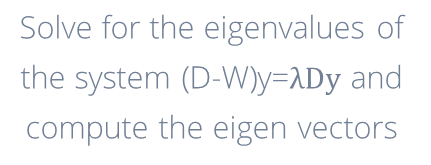
\includegraphics[width=0.55\textwidth]{slide10_eigen_system.png}
    \end{figure}

\end{frame}

% ======================================================================
% SLIDE 11 -- Grouping Algorithm: Step 4
% ======================================================================
\begin{frame}{The Grouping Algorithm --- Step 4: Split graph}

    \begin{itemize}
        \item Once the eigenvectors are computed, we can partition the graph into two pieces using the second smallest eigenvector.
        \item This is done by finding a splitting point (usually 0) and assigning pixels to one group or the other with respect to it.
    \end{itemize}

\end{frame}

% ======================================================================
% SLIDE 12 -- Grouping Algorithm: Step 5
% ======================================================================
\begin{frame}{The Grouping Algorithm --- Step 5: Recursive cut}

    \begin{itemize}
        \item After the graph is broken into two pieces, calculate the \textbf{Ncut} value for the current bipartition; we can recursively run our algorithm on the two partitioned parts.
        \item This is continued till \textbf{Ncut($A$,$b$) $\geq$ threshold value}.
        \item (i.e., the connection between $A$ and $B$ is nearly as strong as their internal volume, thus no clear partitions can be found).
    \end{itemize}

\end{frame}

% ======================================================================
% SLIDE 13 -- Ncut Results
% ======================================================================
\begin{frame}{Ncut Results}

    \centering
    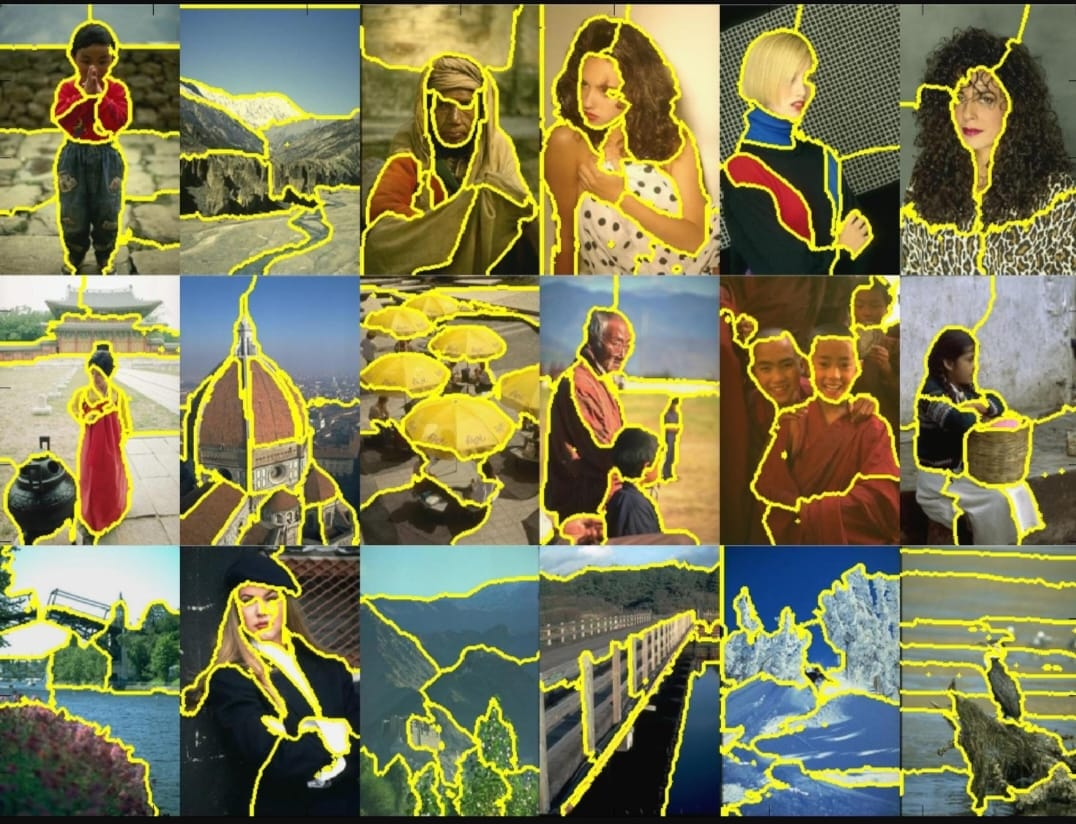
\includegraphics[width=0.85\textwidth,height=0.62\textheight,keepaspectratio]{slide13_ncut_results.jpg}

    \emph{Source: Berkeley segmentation dataset}

\end{frame}

% ======================================================================
% SLIDE 14 -- PRACTICAL APPLICATIONS
% ======================================================================
\begin{frame}{Practical Applications}

    \begin{itemize}
        \item \textbf{Medical Imaging:} Crucial for accurate organ and tumor boundary extraction in complex MRI and CT scans where edges are ambiguous.
        \item \textbf{Autonomous Driving:} Used in scene parsing to differentiate between drivable roads, pedestrians, and obstacles.
        \item \textbf{Interactive Photo Editing:} Enabling intelligent foreground-background separation tools in design software.
    \end{itemize}

    \begin{columns}
        \begin{column}{0.33\textwidth}
            \centering
            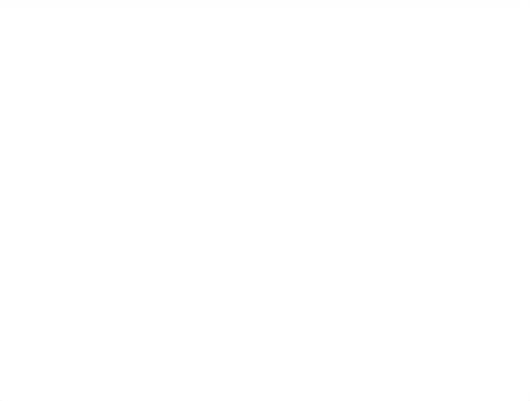
\includegraphics[width=0.7\textwidth]{slide14_medical_imaging.png}
        \end{column}
        \begin{column}{0.33\textwidth}
            \centering
            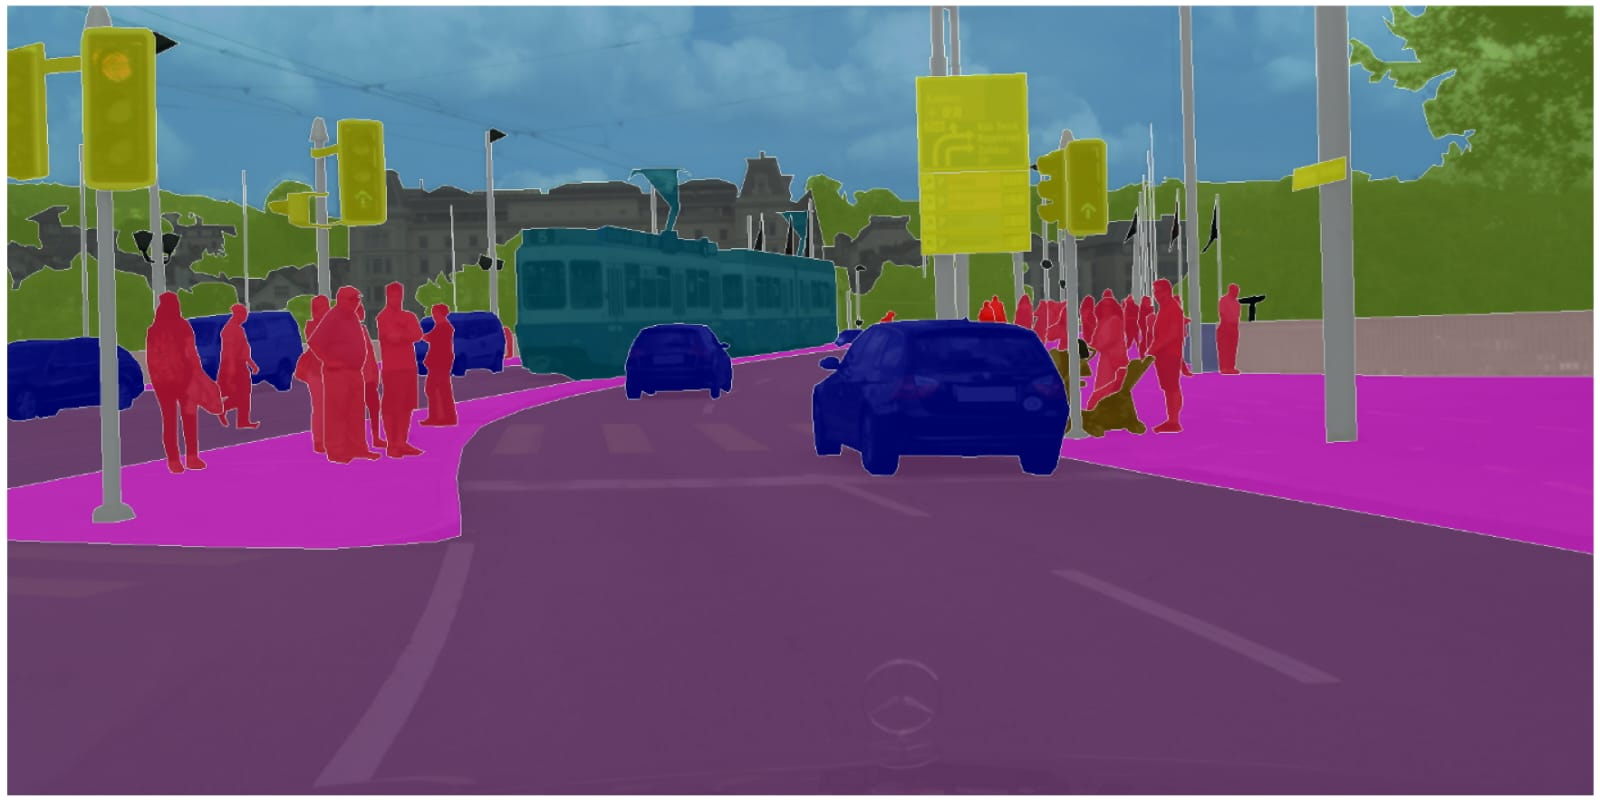
\includegraphics[width=0.7\textwidth]{slide14_autonomous_driving.jpg}
        \end{column}
        \begin{column}{0.33\textwidth}
            \centering
            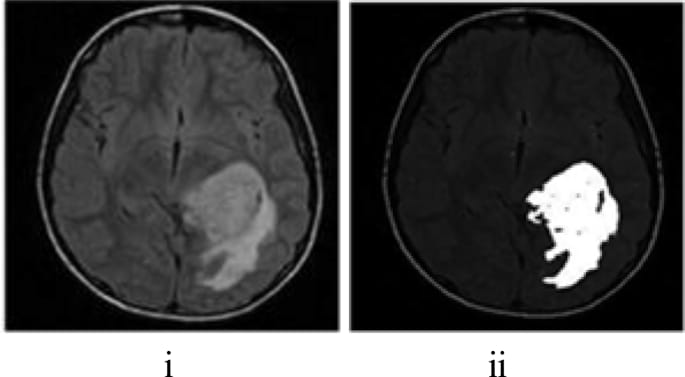
\includegraphics[width=0.7\textwidth]{slide14_photo_editing.jpg}
        \end{column}
    \end{columns}

\end{frame}

% ======================================================================
% SLIDE 15 -- Conclusion
% ======================================================================
\begin{frame}{Conclusion}

    \begin{itemize}
        \item This paper has developed a grouping algorithm based on the view that perceptual grouping should be a process that aims to extract global impressions of a scene and provide a hierarchical description of it.
        \item A computational method based on this idea has been developed and applied to segmentation of brightness, colour and texture.
        \item Results of experiments on real and synthetic images are very encouraging and illustrate that the normalized cut criterion does indeed satisfy our initial goal of extracting the ``big picture'' of a scene.
    \end{itemize}

\end{frame}

% ======================================================================
% Thank you / References
% ======================================================================
\begin{frame}{References}

    \begin{thebibliography}{9}
        \bibitem{shimalik}
        Jianbo Shi and Jitendra Malik,
        \emph{Normalized Cuts and Image Segmentation},
        IEEE Transactions on Pattern Analysis and Machine Intelligence (PAMI), Vol. 22, No. 8, pp. 888--905, August 2000.
    \end{thebibliography}

    \vspace{1cm}
    \centering
    {\Large Thank You}

\end{frame}

\end{document}
